
\section{Conflicts and Coordination}
\label{sec:motivation}

As repositories for application state, databases are traditionally
tasked with maintaining correct data on behalf of users. During
concurrent access to data, a database ensuring correctness must
therefore decide which user operations can execute simultaneously and
which, if any, must coordinate, or block. In this section, we explore
the relationship between the correctness criteria that a database attempts
to maintain and the coordination costs of doing so.

\minihead{By example} As a running example, we consider a
database-backed payroll application that maintains information about
employees and departments within a small business. In the application,
$a.)$ each employee is assigned a unique ID number and $b.)$ each
employee belongs to exactly one department. A database ensuring correctness must
maintain these application-level properties, or \textit{invariants} on
behalf of the application (i.e., without application-level
intervention). In our payroll application, this is non-trivial: for
example, if the application attempts to simultaneously create two
employees, then the database must ensure the employees are
assigned distinct IDs.

\minihead{Serializability and conflicts} The classic answer to
maintaining application-level invariants is to use serializable
isolation: execute each user's ordered sequence of operations, or
\textit{transactions}, such that the end result is equivalent to some
sequential execution~\cite{tamer-book,bernstein-book,gray-virtues}. If
each transaction preserves correctness in isolation, composition via
serializable execution ensures correctness. In our payroll example,
the database would execute the two employee creation transactions such
that one transaction appears to execute after the other, avoiding 
duplicate ID assignment.



While serializability is a powerful abstraction, it comes with a cost:
for arbitrary transactions (and for all implementations of
serializability's more conservative variant---conflict
serializability), any two operations to the same item---at least one
of which is a write---will result in a \textit{read/write
  conflict}. Under serializability, these conflicts require
coordination or, informally, blocking communication between concurrent
transactions: to provide a serial ordering, conflicts must be totally
ordered across transactions~\cite{bernstein-book}. For example, given database state
$\{x=\bot, y=\bot\}$, if transaction $T_1$ writes $x=1$ and reads from
$y$ and $T_2$ writes $y=1$ and reads from $x$, a database cannot both
execute $T_1$ and $T_2$ entirely concurrently and maintain
serializability~\cite{davidson-survey,hat-vldb}.

\minihead{The costs of coordination} The coordination overheads above
incur three primary penalties: increased latency (due to stalled
execution), decreased throughput, and, in the event of partial
failures, unavailability. If a transaction takes $d$ seconds to
execute, the maximum throughput of conflicting transactions operating
on the same items under a general-purpose (i.e., interactive,
non-batched) transaction model is limited by $\frac{1}{d}$, while
coordinating operations will also have to wait. On a single system,
delays can be small, permitting tens to hundreds of thousands of
conflicting transactions per item per second. In a partitioned
database system, where different items are located on different
servers, or in a replicated database system, where the same item is
located (and is available for operations) on multiple servers, the
cost increases: delay is lower-bounded by network latency. On a local
area network, delay may vary from several microseconds (e.g., via
Infiniband or RDMA) to several milliseconds on today's cloud
infrastructure, permitting anywhere from a few hundred transactions to
a few hundred thousand transactions per second. On a wide-area
network, delay is lower-bounded by the speed of light (worst-case on
Earth, around $75$ms, or about 13 operations per
second~\cite{hat-vldb}). Under network
partitions~\cite{queue-partitions}, as delay tends towards infinity,
these penalties lead to unavailability~\cite{gilbert-cap,hat-vldb}. In
contrast, operations executing without coordination can proceed
concurrently and will not incur these penalties.

\minihead{Quantifying coordination overheads} To further understand the
costs of coordination, we performed two sets of measurements---one using
a database prototype and one using traces from
prior studies.




\begin{figure}
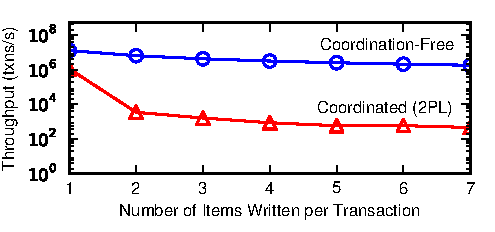
\includegraphics[width=\columnwidth]{figs/micro_thru.pdf}\vspace{-.5em}
\caption{Microbenchmark performance of coordinated and
  coordination-free execution of transactions of varying size writing
  to eight items located on eight separate multi-core servers.}
\label{fig:micro}
\end{figure}

We first compared the throughput of a set of coordinated and
coordination-free transaction execution. We partitioned a set
of eight data items across eight servers and ran one set of
transactions with an optimized variant of two-phase locking (providing
serializability)~\cite{bernstein-book} and ran another set of transactions
without coordination (Figure~\ref{fig:micro}; see
\rappendix{\appexperiment} for more details). With
single-item, non-distributed transactions, the coordination-free
implementation achieves, in aggregate, over 12M transactions per
second and bottlenecks on \textit{physical resources}---namely, CPU
cycles. In contrast, the lock-based implementation achieves
approximately $1.1$M transactions per second: it is unable to fully
utilize all multi-core processor contexts due to lock contention. For
distributed transactions, coordination-free throughput decreases linearly
(as an $N$-item transaction performs $N$ writes), while the throughput
of coordinating transactions drops by over three orders of
magnitude.



While the above microbenchmark demonstrates the costs of a particular
\textit{implementation} of coordination, we also studied the
effect of more fundamental, implementation-independent overheads
(i.e., also applicable to optimistic and scheduling-based concurrency
control mechanisms). We determined the maximum attainable throughput
for coordinated execution within a single datacenter (based on data
from~\cite{bobtail}) and across multiple datacenters (based on data
from~\cite{hat-vldb}) due to blocking coordination during atomic
commitment~\cite{bernstein-book}. For an $N$-server transaction,
classic two-phase commit (\cpc) requires $N$ (parallel) coordinator to
server RTTs, while decentralized two-phase commit (\dpc) requires $N$
(parallel) server to server broadcasts, or $N^2$
messages. Figure~\ref{fig:2pc} shows that, in the local area, with
only two servers (e.g., two replicas or two coordinating operations on
items residing on different servers), throughput is bounded by $1125$
transactions/s (via \dpc; $668$/s via \cpc). Across eight servers,
\dpc throughput drops to $173$ transactions/s (resp. $321$ for \cpc)
due to long-tailed latency distributions. In the wide area, the
effects are more stark: if coordinating from Virginia to Oregon, \dpc
message delays are $83$~ms per commit, allowing $12$ operations per
second. If coordinating between all eight EC2 availability zones,
throughput drops to slightly over $2$ transactions/s in both
algorithms. (\rappendix{\appexperiment} provides more details.)

These results should be unsurprising: coordinating---especially over
the network---can incur serious performance penalties. In contrast,
coordination-free operations can execute without incurring these
costs. The costs of actual workloads can vary: if coordinating
operations are rare, concurrency control will not be a bottleneck. For
example, a serializable database executing transactions with disjoint
read and write sets can perform as well as a non-serializable database
without compromising correctness~\cite{shore-communication}. However,
as these results demonstrate, minimizing the amount of coordination
and its degree of distribution can therefore have a tangible impact on
performance, latency, and
availability~\cite{pacelc,hat-vldb,gilbert-cap}. While we study real
applications in Section~\ref{sec:evaluation}, these measurements
highlight the worst of coordination costs on modern hardware.

\begin{figure}
  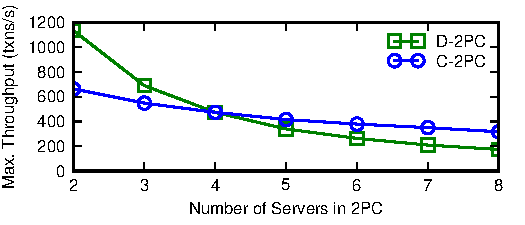
\includegraphics[width=\columnwidth]{figs/singledc-twopc.pdf}\\
  {\centering \textbf{\scriptsize a.) Maximum transaction
      throughput over local-area network in~\cite{bobtail}}\par}
  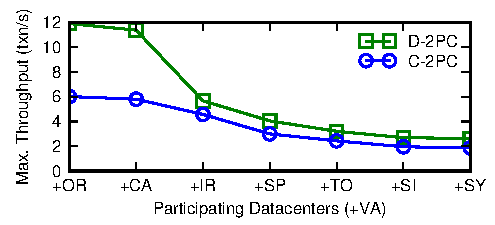
\includegraphics[width=\columnwidth]{figs/multidc-twopc.pdf}\\
  \textbf{\scriptsize b.) Maximum throughput over wide-area network
    in~\cite{hat-vldb} with transactions originating from a
    coordinator in Virginia (VA; OR:~Oregon, CA:~California,
    IR:~Ireland, SP:~S\~{a}o Paulo, TO:~Tokyo, SI:~Singapore,
    SY:~Sydney)}

\caption{Atomic commitment latency as an upper bound on throughput
  over LAN and WAN networks.}
\label{fig:2pc}
\end{figure}


\minihead{Our goal: Minimize coordination} In this paper, we seek to
minimize the amount of coordination required to correctly execute an
application's transactions. As discussed in Section~\ref{sec:intro},
serializability is \textit{sufficient} to maintain correctness but is
not always \textit{necessary}; that is, many---but not
all---transactions can be executed concurrently without necessarily
compromising application correctness. In the remainder of this paper,
we identify when safe, coordination-free execution is possible. If
serializability requires coordinating between each possible pair of
conflicting reads and writes, we will only coordinate between pairs of
operations that might compromise \textit{application-level}
correctness. To do so, we must both raise the specification of
correctness beyond the level of reads and writes and directly account
for the process of reconciling the effects of concurrent transaction
execution at the application level.


